\documentclass{article}
\usepackage[utf8]{inputenc}
\usepackage{wasysym}
\usepackage{qrcode}
\usepackage[colorlinks]{hyperref}
\usepackage{lmodern}
\usepackage{graphicx}
\usepackage{xcolor}
\usepackage[left=2cm, top=3cm, right=2cm]{geometry}
\usepackage{booktabs}
\usepackage{svg}
\usepackage{minted}
\usepackage{xcolor}
\definecolor{LightGray}{gray}{0.975}

%setup new colors
\hypersetup{
%linkcolor=blue
%,citecolor=
%,filecolor=
urlcolor=blue
%,menucolor=
%,runcolor=
%,linkbordercolor=
%,citebordercolor=
%,filebordercolor=
%,urlbordercolor=
%,menubordercolor=
%,runbordercolor=
}

\title{Database Administration \\ Lab 08: SQL Functions.}
\author{Andrés Calderón, Ph.D.}
\date{\today}

\begin{document}

\maketitle

\section{Introduction}
In this lab, we will take a hands-on approach to explore data analysis using SQL functions within the context of European football leagues. Working with a rich dataset that spans multiple seasons and thousands of players and matches, you will gain practical experience designing SQL functions that summarize meaningful insights from relational data.

The lab focuses on two key analytical tasks: querying match outcomes based on league, season, and stage; and ranking players by performance attributes. These exercises are designed to deepen your understanding of SQL function creation, data aggregation, and conditional logic—all essential tools for database administrators and data analysts alike.

By the end of this lab, you will have written reusable and adaptable SQL functions, reinforced your ability to work with foreign key relationships, and built confidence in extracting actionable insights from a real-world sports dataset.

\section{Getting Some Data}
This time, we will work with European football leagues, specifically 11 leagues from countries such as England, France, and the Netherlands. The database contains data from the 2008 to 2016 seasons, covering more than 25,000 matches and 10,000 players.
More information about the database can be found at \url{https://www.kaggle.com/datasets/hugomathien/soccer}. The dataset we will use is a simplified version that includes only a few player attributes and no team attributes. Figure \ref{fig:erd} shows the Entity-Relationship Diagram (ERD) of the database.

You can download the data for the database \href{https://drive.google.com/drive/folders/12KoKu76ZDpIoDtE78Lc6g6Y2y0zTJJbO?usp=sharing}{here}. Please follow these steps:

\begin{enumerate}
    \item Create a database named \textit{euroleagues}.
    \item Connect to the database.
    \item Download and run the \texttt{Euroleagues\_ddl.sql} file to create the database schema.
    \item Download and save the 6 TSV files from the \textbf{data} folder to an accessible location.
    \item Download and run the \texttt{Euroleagues\_copy.sql} file. Be sure to update the file paths according to your operating system and the location of the TSV files.
    \item Enjoy!
\end{enumerate}

\begin{figure}
 \centering
 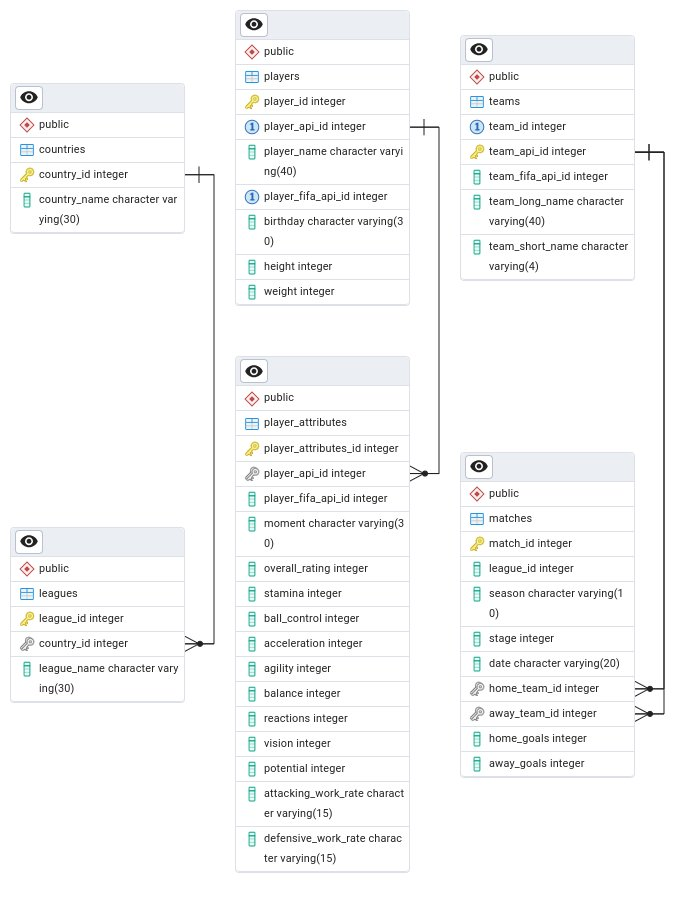
\includegraphics[width=0.75\textwidth]{figures/Euroleagues_erd.jpg}
 \caption{E-R Diagram of the Euroleagues Database.}
 \label{fig:erd}
\end{figure}

\section{Working on Functions}
We will apply what we’ve learned to code a couple of functions that summarize interesting facts from the database. Specifically, you will create functions for:

\begin{enumerate}
    \item A function to display the match results for a particular league, season, and stage. That is, given a \textit{season} and a \textit{stage} from the \texttt{matches} table, you will select all the games for a specific league (\textit{league\_id}). Note that you may need to assume or explicitly enforce a foreign key constraint between the \texttt{matches} and \texttt{leagues} tables. If a value of 0 is passed for the league, the function should generate the report for all applicable leagues.

    \item Given a particular year and a numeric player attribute, you will create a ranking of the Top 10 players in descending order based on that attribute for the specified year. If no attribute is provided, the function should generate a ranking for all numeric player attributes.  If a player has multiple measurements for an attribute in the same year, you should use the average value.
\end{enumerate}

\section{What We Expect}
You will submit a well-structured report in \textbf{PDF} format, presenting your work and describing the code of your functions, along with any relevant information you consider appropriate. Include a couple of examples that you used to validate your results. Along with the report, submit plain text files containing the code for both functions (please use \textbf{.sql} extensions). Package everything into a single \textbf{ZIP} file and send it to my email before \textbf{April 14, 2025}, with the subject line: {\LARGE \textbf{\texttt{[DBA] Lab 08}}}.

\vspace{5mm}
Happy Hacking \includesvg[width=4mm]{figures/sunglasses}!

\end{document}

